%%%%%%%%%%%%%%%%%%%%%%%%%%%%%%%%%%%%%%%%%%%%%%%%%%%%%%%%%%%%%%%%%%%%%%
%%                     Dissociation
%%%%%%%%%%%%%%%%%%%%%%%%%%%%%%%%%%%%%%%%%%%%%%%%%%%%%%%%%%%%%%%%%%%%%%
%\color{blue}
\subsection{Glyph: \glyph{Dissociation}}\label{sec:dissociation}

The dissociation of a EPN into two EPNs represents the rupture of a non-covalent binding between the biological entities represented by those EPNs.

\begin{glyphDescription}
 \item[SBO]\mbox{}\\ SBO:0000180 ! dissociation
 \item[origin]\mbox{}\\ One \glyph{consumption} arc (section \ref{sec:consumption}).
 \item[target]\mbox{}\\  More than one \glyph{production} arc (section \ref{sec:production}).
 \item[node]\mbox{}\\ A \glyph{dissociation} between several entities is represented by two concentric empty discs. A simple empty disc could be, in some cases, confused with the \glyph{modulation} (section \ref{sec:modulation}).
 \end{glyphDescription}


\begin{figure}[H]
  \centering
  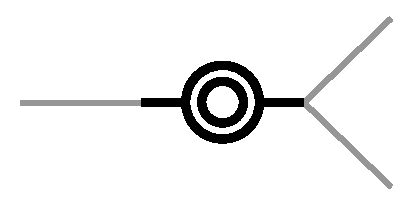
\includegraphics[scale = 0.5]{images/dissociation}
  \caption{The \PD glyph for \glyph{dissociation}.}
  \label{fig:dissociation}
\end{figure}
